\documentclass[runningheads]{llncs}
\usepackage[T1]{fontenc}
\usepackage{graphicx}
\usepackage{booktabs}
\usepackage{amsmath,amssymb}
\usepackage{multirow}
\usepackage{xurl}
\usepackage{xcolor}
\usepackage{enumitem}
\usepackage{float}
\usepackage{placeins}
\graphicspath{{figures/}}
\emergencystretch=1em
\setlist{nosep}
\setlist[itemize]{label=\textbullet}
\setlength{\textfloatsep}{7pt plus 2pt minus 1pt}
\setlength{\floatsep}{6pt plus 2pt minus 1pt}
\setlength{\intextsep}{6pt plus 2pt minus 1pt}
\renewenvironment{center}{\raggedright}{\par}

\begin{document}
\raggedright

\title{SafetyPool: Guided Exploration for Deep Reinforcement Learning}
\titlerunning{SafetyPool: Guided Exploration for Deep Reinforcement Learning}

\author{Sai Durga Karthik Nandiraju \and Manolo Dulva Hina}
\authorrunning{Karthik Nandiraju and Manolo Dulva Hina}
\institute{ECE Paris, OMNES Education, Paris, France}

\maketitle

\begin{abstract}
Exploration is necessary in deep reinforcement learning, but random actions can create avoidable collisions in driving simulations. We present SafetyPool, a Deep Q-Network (DQN) training framework that stores local evidence about previously visited states and uses this evidence to block actions associated with near-term hazards during exploration. The learned network is evaluated without a safety mask, so test performance measures the frozen policy rather than an external controller. We compare SafetyPool against Epsilon-Greedy DQN, NoisyNet DQN, and DQN with Random Network Distillation in MetaDrive and HighwayEnv. Each environment-specific analysis uses 23 matched training seeds, 500 training episodes, and 300 test episodes per seed. Collision Restricted Mean Survival Time (RMST) through the fixed 500-step test window is the sole reported outcome. In MetaDrive, SafetyPool obtains a Collision RMST interquartile mean (IQM) of 229.8 steps, compared with 91.4, 92.1, and 91.6 for the baselines. In the matched 23-seed Highway subset, the corresponding IQMs are 122.15, 5.79, 5.68, and 6.44 steps. Paired Wilcoxon comparisons remain significant against all three baselines after Holm correction in both environment-specific analyses.

\keywords{Deep reinforcement learning \and autonomous driving \and safe exploration \and collision RMST \and survival analysis}
\end{abstract}

\section{Introduction}

Reinforcement learning (RL) trains an agent by allowing it to interact with an environment and learn from rewards and penalties \cite{sutton2018reinforcement}. Deep reinforcement learning (DRL) uses a neural network to represent the agent's decision rule. In autonomous-driving research, DRL can discover behaviours that are difficult to specify manually, but learning requires exploration: the agent must sometimes try an action whose outcome is uncertain. A randomly selected steering or acceleration command may therefore cause an autonomous vehicle collision or send the vehicle off the road.

This paper investigates whether exploration can be guided by state-specific safety evidence. The proposed algorithm, SafetyPool, extends a Deep Q-Network (DQN). During training, SafetyPool groups similar observations into state pools, records which actions have produced sufficient safe or hazardous evidence, and prevents well-supported hazardous actions from being selected. During testing, this intervention is removed and the frozen DQN selects the action with the largest predicted action-value. This separation matters: a test-time shield can make a weak policy appear safe, whereas our evaluation asks whether guided training changes the policy itself.

We address the following research questions:

\begin{itemize}[leftmargin=1.8em,labelindent=0pt,labelsep=0.5em,itemsep=0.25em,topsep=0.25em]
\item \textit{RQ1:} Does SafetyPool delay or prevent autonomous vehicle collisions relative to common exploration baselines?
\item \textit{RQ2:} Are the observed improvements consistent across random seeds and statistically supported?
\item \textit{RQ3:} How should the Collision RMST improvement be interpreted?
\end{itemize}

The contributions of this paper are as follows:

\begin{itemize}[leftmargin=*]
\item an evidence-guided exploration mechanism that separates temporary state candidates, promoted state pools, retired pools, and a bounded hazard memory;
\item environment-specific evaluations in MetaDrive and HighwayEnv over 23 matched seeds and 6,900 test episodes per method, against Epsilon-Greedy DQN, NoisyNet DQN, and DQN with Random Network Distillation (RND); and
\item a Collision RMST analysis supported by robust aggregation, confidence intervals, and matched-seed tests.
\end{itemize}

The rest of this paper is structured as follows. Section~2 discusses the background and related work. Section~3 presents SafetyPool, Section~4 describes the experimental design, and Section~5 reports and discusses the results. Section~6 concludes the paper and outlines future work.

\section{Background and Related Work}

\subsection{Value-based reinforcement learning and exploration}

An RL problem is commonly formalised as a Markov decision process (MDP), consisting of states, actions, transition probabilities, rewards, and a discount factor \cite{sutton2018reinforcement}. Q-learning estimates the expected discounted return of choosing action $a$ in state $s$ \cite{watkins1992qlearning}. A DQN approximates this action-value function, $Q(s,a)$, with a neural network \cite{mnih2015human}. Double DQN reduces overestimation \cite{hasselt2016double}; duelling networks separate state value from action advantage \cite{wang2016dueling}; prioritised replay samples informative transitions more frequently \cite{schaul2016prioritized}; and Rainbow combines several such improvements \cite{hessel2018rainbow}.

Exploration methods decide how the learner gathers experience. Epsilon-Greedy chooses a random action with probability $\epsilon$. NoisyNet injects learned noise into network parameters \cite{fortunato2018noisy}. RND supplies intrinsic reward when a fixed random network is difficult for a predictor to imitate \cite{burda2018rnd}. Other approaches use visitation counts \cite{bellemare2016count}, prediction error \cite{pathak2017curiosity}, and bootstrapped value functions \cite{osband2016bootstrapped}. These methods promote novelty or uncertainty; they do not necessarily distinguish an informative action from a repeatedly hazardous one.

SafetyPool advances this line of work by making empirical state--action outcomes part of the exploration decision rather than relying only on novelty, uncertainty, or a fixed constraint. It guides the experiences collected by the DQN during training while leaving the learned policy to act independently during evaluation. Table~\ref{tab:related} positions SafetyPool relative to representative exploration and safety approaches by comparing their training-time exploration, source of safety knowledge, and evaluation behaviour.

\begin{table}[H]
\caption{Relationship between SafetyPool and representative exploration and safety approaches. Evaluation behaviour shows whether the learned policy acts directly or an auxiliary mechanism may override it.}
\label{tab:related}
\raggedright
\setlength{\tabcolsep}{4pt}
\begin{tabular}{p{1.8cm}p{3.8cm}p{4.8cm}}
\toprule
Approach & Training guidance & Safety knowledge and evaluation role \\
\midrule
Epsilon-Greedy & Random action with probability $\epsilon$ & No safety knowledge; learned DQN acts directly during evaluation \\
NoisyNet & Learned parameter noise & No safety knowledge; learned DQN acts directly during evaluation \\
RND & Prediction-error novelty bonus & No safety knowledge; learned DQN acts directly during evaluation \\
Formal shield & Base explorer constrained by logical rules & Hand-specified safety rules; shield may override the policy \\
Recovery policy & Base policy plus recovery controller & Learned risk model; recovery controller may override the policy \\
\textbf{SafetyPool} & Matched-state outcome evidence guides selection among safe and unknown actions & Empirical action outcomes; SafetyPool is disabled and the frozen DQN acts directly during evaluation \\
\bottomrule
\end{tabular}
\end{table}

\subsection{Safety mechanisms}

Safe RL includes constrained optimisation, risk-sensitive objectives, external shields, recovery policies, and action correction \cite{garcia2015safe}. Constrained MDPs represent safety as an explicit cost budget \cite{altman1999cmdp}; constrained policy optimisation seeks approximately feasible policy updates \cite{achiam2017cpo}. Shielding rejects actions that violate a formal safety specification \cite{alshiekh2018shielding}, while safety layers correct continuous actions using learned constraints \cite{dalal2018safetylayer}. Recovery RL learns a separate policy for leaving unsafe regions \cite{thananjeyan2021recovery}, and Lyapunov methods enforce stability-style constraints \cite{chow2018lyapunov}. In contrast, SafetyPool uses empirical, local evidence to guide exploration only during training. It neither assumes a formal vehicle-dynamics model nor uses an external test-time shield.

\subsection{Autonomous-driving simulation and evaluation}

DRL has been widely explored for autonomous driving \cite{kiran2022survey,sallab2017drl,kendall2019driving}. MetaDrive supports configurable procedural driving scenarios and standardised agent interaction \cite{li2023metadrive}, while HighwayEnv provides a lane-based highway simulator with controllable traffic and vehicle dynamics. Reward shaping can accelerate learning by providing informative feedback when the original reward is sparse. However, poorly designed shaping terms can redirect the policy toward maximising a proxy reward instead of the intended driving objective \cite{ng1999shaping}. We therefore evaluate collision-free time directly rather than using reward as the outcome.

Reliable RL comparisons require more than a mean over a few runs. Henderson et al. document sensitivity to implementation and random seeds \cite{henderson2018matters}; Agarwal et al. recommend robust aggregate statistics such as the interquartile mean (IQM) and stratified bootstrap confidence intervals \cite{agarwal2021precipice}; Colas et al. discuss appropriate statistical testing \cite{colas2019empirical}; and Patterson et al. emphasise transparent empirical design \cite{patterson2024empirical}. Our analysis combines robust aggregation with matched-seed paired tests because the IQM limits the influence of unusually high or low seed outcomes, while pairing compares methods under the same training randomisations. Together, these choices make the comparison more sensitive to method differences and less sensitive to seed-specific variation.

\section{Methodology}

\subsection{Base learner}

The agent receives a vector observation $s_t$ at time $t$ and selects one of nine discrete actions formed by three steering choices and three throttle/brake choices. A DQN with parameters $\theta$ predicts one action-value for each action. The temporal-difference target is
\begin{equation}
y_t=r_t+\gamma(1-d_t)\max_{a'}Q_{\theta^-}(s_{t+1},a'),
\end{equation}
where $r_t$ is the reward, $\gamma=0.99$ is the discount factor, $d_t$ is one when the episode ends, and $\theta^-$ denotes the target network. The online network minimises the squared difference between $y_t$ and $Q_\theta(s_t,a_t)$. Optimisation uses Adam \cite{kingma2015adam}, whose adaptive learning rates are based on first- and second-moment estimates. Neural-network gradients are computed by back-propagation \cite{rumelhart1986backprop}.

\subsection{State candidates, active pools, and hazard memory}

SafetyPool maintains bounded memory at three levels.

\textbf{Candidate states} are newly observed state regions. A candidate must be revisited four times before promotion, which reduces the chance that a single noisy observation creates a permanent rule. At most 150 candidates are retained; eviction begins above a soft limit of 125.

\textbf{Active state pools} are promoted regions with action-level evidence. A pool stores a representative state, visit counts, observed outcomes, and whether each action is currently considered safe, hazardous, or insufficiently known. The active collection is capped at 500 pools. Retired pools preserve summaries of displaced regions.

\textbf{Hazard memory} retains up to 125 hazardous summaries even when their original pools are removed. This makes repeated severe outcomes less likely to be forgotten simply because memory capacity is reached.

Two observations are considered for the same region only when they pass both a directional and a magnitude gate. Directional similarity is measured by cosine similarity,
\begin{equation}
\operatorname{cos}(x,z)=\frac{x^\top z}{\lVert x\rVert_2\lVert z\rVert_2},
\end{equation}
and magnitude discrepancy is measured by root-mean-square (RMS) difference. Candidate matching requires cosine similarity of at least 0.90 and RMS difference of at most 0.25; active-pool matching uses 0.90 and 0.20. Thresholds are calibrated from up to 3,000 observed states, with at most 20,000 state pairs.

\subsection{Evidence-guided action selection}

For a matched pool, an action is blocked only after its recorded outcomes provide sufficient hazard evidence. Safety confirmation requires at least two supporting visits and checks a five-step horizon with a minimum progress threshold of 0.01. Blocking persists for a short warning window of two decisions. If no state matches, if evidence is missing, or if all evidence is inconclusive, the algorithm falls back to the base exploration rule rather than inventing a safety label.

Training proceeds in three interpretable stages:

\begin{enumerate}[leftmargin=*]
\item \textbf{Initial evidence collection.} The learner attempts non-blocked actions in matched regions so that each locally available action receives evidence.
\item \textbf{Guided learning.} For the main training phase, approximately 80\% of eligible choices use the DQN-preferred safe action and 20\% explore an action that remains unknown. If no unknown action exists, the greedy safe action is used.
\item \textbf{Policy consolidation.} In the final 20\% of training, pool-based action selection is disabled and the DQN acts greedily. This phase forces the neural policy to operate without continued assistance from the state memory.
\end{enumerate}

If every action is blocked, SafetyPool selects the action with the least recorded risk; otherwise the vehicle could become undefined at the exact moment a decision is required. During testing, all state-pool masks and safety scans are disabled. The final trained network is frozen and uses $\arg\max_a Q_\theta(s,a)$ at every step.

\section{Experimental Design}

\subsection{Environments, methods, and protocol}

Experiments use MetaDrive \cite{li2023metadrive} and HighwayEnv. MetaDrive uses three procedural map blocks, traffic density 0.2, and nine discrete controls. HighwayEnv uses the \texttt{highway-v0} environment, a flattened normalised Kinematics observation, traffic density 0.2, and the same nine-action acceleration--steering grid. Collisions and leaving the road receive penalties of 50. Each method is trained for 500 episodes and tested for 300 episodes through a fixed 500-step observation horizon. Training uses a replay capacity of 50,000, batch size 64, learning rate $5\times10^{-5}$, hidden width 128, discount factor 0.99, and target-network update interval 1,000. Testing is deterministic, starts from scenario seed 100000, freezes the network, and uses greedy DQN actions without SafetyPool lookup or masking.

The MetaDrive analysis uses 23 matched training seeds: \small 3, 5, 7, 9, 13, 17, 19, 29, 31, 33, 38, 42, 45, 48, 54, 63, 67, 69, 77, 85, 94, 108, and 111.\normalsize
The Highway subset analysis uses 23 matched training seeds: \small 3, 5, 7, 9, 13, 17, 27, 33, 38, 42, 45, 48, 54, 63, 65, 67, 69, 73, 76, 77, 93, 108, and 111.\normalsize
Within each environment, the same seed list and test scenarios are used for SafetyPool, Epsilon-Greedy DQN, NoisyNet DQN, and DQN+RND. Each environment--method combination therefore contributes 6,900 test episodes. The Highway analysis is explicitly reported as the matched 23-seed subset supplied with the reproducibility archive.

\subsection{Outcome measures}

\textbf{Collision Restricted Mean Survival Time (RMST)} is the sole outcome reported in this study. A collision event occurs when the controlled ego vehicle strikes another vehicle or a road object. The first collision time is treated as the event time. An episode without a collision during observation is right-censored: it contributes all observed collision-free time, but the analysis does not extrapolate beyond the fixed horizon. The Kaplan--Meier estimator \cite{kaplan1958nonparametric} calculates the probability of remaining collision-free at each step. Collision RMST is the area under the estimated survival function up to $\tau=500$:
\begin{equation}
\operatorname{RMST}(500)=\int_0^{500}\widehat{S}(t)\,dt,
\end{equation}
where $\widehat{S}(t)$ is the estimated probability of remaining collision-free through step $t$. Higher RMST is better. Its units are environment steps, so an RMST of 229.8 represents about 229.8 collision-free steps on average within the common observation window \cite{royston2013rmst}. The estimate uses both early collision events and right-censored episodes.

The fixed horizon gives every method the same observation window and prevents extrapolation beyond the collected data. A collision at step 40 contributes much less collision-free time than one at step 400. An episode without a collision contributes its complete observed duration and is censored at the horizon. A method obtains a larger RMST when collisions occur later or when more episodes remain collision-free throughout observation.

\subsection{Statistical analysis}

For each method, we aggregate the 23 seed-level results with IQM, which sorts the seed values, discards the lowest and highest quarters, and averages the central half. IQM is more resistant to unusually good or bad seeds than the ordinary mean \cite{agarwal2021precipice}. A 95\% confidence interval (CI) is obtained by resampling the 23 seeds with replacement, recomputing the IQM for each bootstrap sample, and taking the 2.5th and 97.5th percentiles \cite{efron1979bootstrap}.

For SafetyPool-versus-baseline inference, we apply a two-sided Wilcoxon signed-rank test to the matched seed-level Collision RMST values \cite{wilcoxon1945rank}. For each environment, the three SafetyPool-versus-baseline $p$-values are corrected together using Holm's step-down method \cite{holm1979procedure}. We call a comparison statistically supported when the corrected $p$-value is below 0.05.

The paired design compares methods trained with the same seed. It therefore asks whether SafetyPool tends to improve on a baseline under matched training randomisation, rather than comparing unrelated collections of runs. The IQM summarises the central half of the 23 seed results, the bootstrap interval describes uncertainty in that aggregate, and the paired test evaluates the direction and consistency of the seed-level differences.

\section{Results and Discussion}

\subsection{Collision RMST outcomes}

Table~\ref{tab:aggregate} reports Collision RMST only. In MetaDrive, SafetyPool's IQM is 229.8 steps, compared with approximately 91--92 steps for every baseline. In the matched 23-seed Highway subset, SafetyPool reaches 122.15 steps, compared with 5.79 for Epsilon-Greedy, 5.68 for NoisyNet, and 6.44 for RND. Figures~\ref{fig:metadrive_iqm} and \ref{fig:highway_iqm} show the environment-specific aggregate estimates.

\begin{table}[t]
\caption{Collision RMST over 23 matched seeds in each environment: IQM with seed-bootstrap 95\% CI. Higher is better.}
\label{tab:aggregate}
\raggedright
\scriptsize
\resizebox{\textwidth}{!}{\begin{tabular}{lllll}
\toprule
Environment & SafetyPool & Epsilon-Greedy & NoisyNet & RND \\
\midrule
MetaDrive & \textbf{229.8 [151.1, 333.6]} & 91.4 [91.0, 93.1] & 92.1 [87.7, 129.8] & 91.6 [90.9, 93.2] \\
HighwayEnv matched subset & \textbf{122.15 [6.63, 310.14]} & 5.79 [5.64, 46.57] & 5.68 [5.66, 6.54] & 6.44 [5.68, 120.67] \\
\bottomrule
\end{tabular}}
\end{table}

\begin{figure}[t]
\raggedright
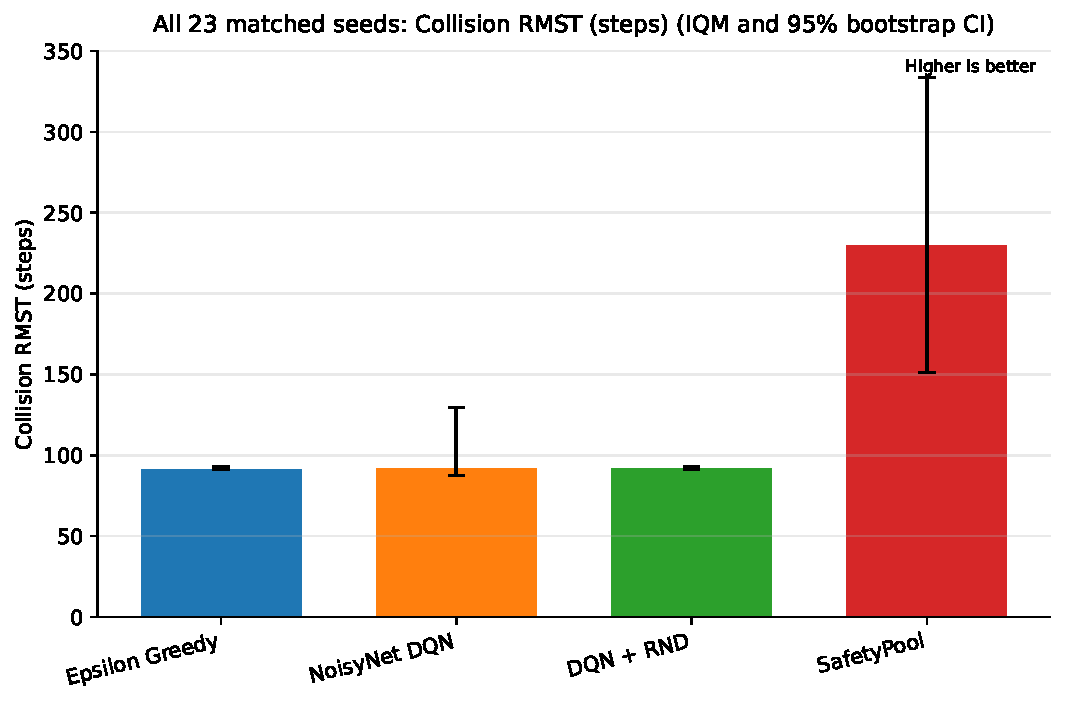
\includegraphics[width=0.66\textwidth]{figure_01_collision_rmst_iqm_ieee_palette.pdf}
\caption{MetaDrive Collision RMST across 23 matched seeds. Bars show IQMs and error bars show seed-bootstrap 95\% CIs. Higher is better.}
\label{fig:metadrive_iqm}
\end{figure}

\begin{figure}[t]
\raggedright
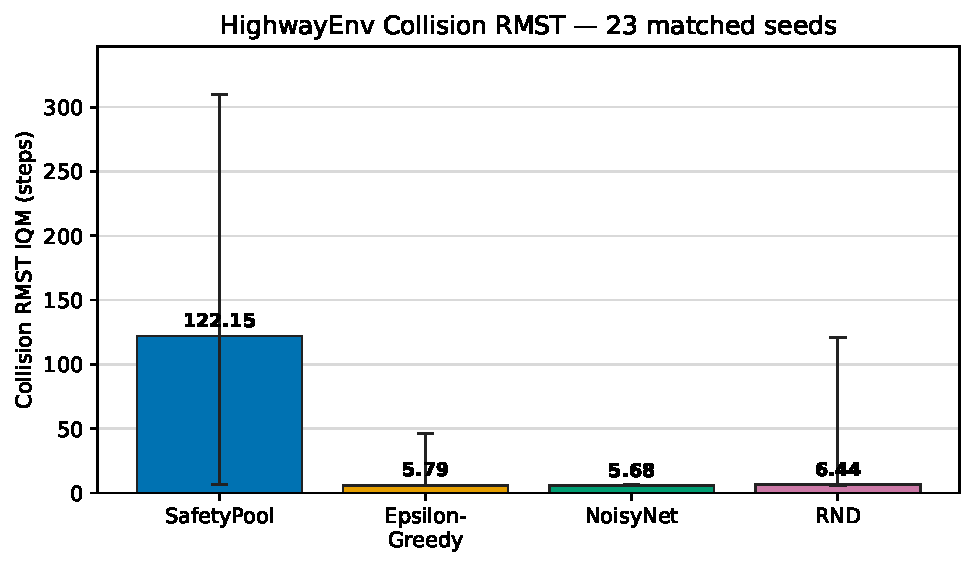
\includegraphics[width=0.66\textwidth]{figure_02_highway_collision_rmst_iqm.pdf}
\caption{HighwayEnv Collision RMST in the matched 23-seed subset. Bars show IQMs and error bars show seed-bootstrap 95\% CIs. Higher is better.}
\label{fig:highway_iqm}
\end{figure}

Table~\ref{tab:tests} gives the Holm-corrected matched-seed comparisons. In MetaDrive, SafetyPool is supported against all three baselines with corrected $p$-values of 0.000024, 0.001885, and 0.000024. The Highway subset result is also supported against all three baselines, with corrected $p$-values of 0.0174, 0.0174, and 0.0171.

\begin{table}[t]
\caption{Collision RMST matched-seed tests. Values are Holm-corrected two-sided Wilcoxon $p$-values.}
\label{tab:tests}
\raggedright
\scriptsize
\setlength{\tabcolsep}{5pt}
\resizebox{\textwidth}{!}{\begin{tabular}{llll}
\toprule
Environment & vs Epsilon-Greedy & vs NoisyNet & vs RND \\
\midrule
MetaDrive & 0.000024 & 0.001885 & 0.000024 \\
HighwayEnv matched subset & 0.0174 & 0.0174 & 0.0171 \\
\bottomrule
\end{tabular}}
\end{table}

All inferential tests include every seed in the environment-specific lists in Sect.~4.1. The Highway intervals are wide because seed-level performance is heterogeneous. The paired tests and aggregate intervals answer different questions: the paired tests use within-seed differences, while the intervals quantify uncertainty in each separate IQM. The Highway result should therefore be read as evidence for the stated matched 23-seed subset, not as a claim about every seed available in the larger uploaded archive.

\subsection{Behaviour of the state memory}

Runtime logs show state-pool and action-mask activity during the evidence-collection and guided phases, while the final consolidation phase deliberately removes pool-based action selection. This schedule transfers control to the learned network before the frozen-policy test and confirms that the guided-exploration mechanism was active during training.

\subsection{Answers to the research questions}

\begin{itemize}[leftmargin=1.8em,labelindent=0pt,labelsep=0.5em,itemsep=0.25em,topsep=0.25em]
\item \textit{RQ1:} SafetyPool increases Collision RMST relative to all three baselines in both environment-specific 23-seed analyses.
\item \textit{RQ2:} The paired Collision RMST improvement is supported for all three baseline comparisons after Holm correction in MetaDrive and in the matched Highway subset.
\item \textit{RQ3:} The result means that SafetyPool delays the first collision or remains collision-free for longer within the same fixed observation horizon.
\end{itemize}

The likely mechanism is selective experience acquisition. Unlike novelty-based exploration, SafetyPool records local action outcomes and directs exploration toward actions that remain unknown without repeatedly selecting actions supported as hazardous. The final pure-DQN phase then transfers control from explicit memory to the value network.

\FloatBarrier
\section{Conclusion and Future Work}

This study evaluated SafetyPool, an evidence-guided exploration method for a DQN driving agent. In MetaDrive, SafetyPool increases Collision RMST from approximately 91--92 baseline steps to 229.8 steps over 23 matched seeds. In the matched 23-seed Highway subset, SafetyPool obtains 122.15 steps compared with 5.79, 5.68, and 6.44 for Epsilon-Greedy, NoisyNet, and RND. Every environment-specific paired comparison is supported after Holm correction. These results show that guided exploration can extend collision-free operation after the safety memory is removed and the frozen DQN acts independently.

Future work will pre-register and evaluate broader Highway seed sets, repeat the analysis across additional traffic configurations, and tune candidate-promotion visits, root-mean-square (RMS) distance thresholds, hazard-pool settings, and eviction criteria. Maximum-step completion, collisions per 1,000 steps, route completion, out-of-road events, and computational cost will be evaluated as separate secondary outcomes rather than mixed with the Collision RMST claim. We will also study additional safety metrics informed by recent safe-learning and safety-critical driving research \cite{brunke2022safe,zhao2022zeroviolation,ji2023safetygymnasium,zhang2023cat,ji2024omnisafe}.

\section*{Data Availability}

The accompanying reproducibility folder contains the exact SafetyPool policies, Highway and MetaDrive frameworks, collision-event episode data, seed-level Collision RMST tables, analysis code, figures, and environment records. The environment-specific 23-seed lists are given in Sect.~4.1.

\section*{Ethical and Safety Statement}

The experiments are simulation-only. Future physical testing should use independent supervision, controlled facilities, formal risk assessment, and applicable transport and research requirements.

% Sequential numbering by first citation, as requested in the review notes.
\begingroup
\scriptsize
\setlength{\itemsep}{0pt}
\bibliographystyle{unsrt}
\bibliography{references}
\endgroup
\end{document}
